%\documentclass[sigconf,anonymous,review]{webmedia}
\documentclass[sigconf]{webmedia}

% \usepackage{lmodern}
%webmeda.cls is adapted from acmart.cls for use in Proceedings of the Brazilian Symposium on Multimedia and the Web (WebMedia)

%% SBC
% \usepackage{graphicx,url}
% \usepackage{subcaption}
% \usepackage{float}
\usepackage[brazil]{babel}
% \usepackage[utf8]{inputenc}  
\usepackage{tabularx}
% \usepackage{booktabs}
% \usepackage{caption}
% \usepackage{amsmath}
% \usepackage{amssymb}
\usepackage{threeparttable}
% \usepackage[hidelinks]{hyperref}
%%

\usepackage{booktabs}
\usepackage{array}
\usepackage{pifont}
\newcommand{\cmark}{\ding{51}}
\newcommand{\xmark}{\ding{55}}
\newcommand{\pmark}{Parcial}
\newcommand{\nmark}{N/A}

%%
%% \BibTeX command to typeset the BibTeX logo in the docs
\AtBeginDocument{%
  \providecommand\BibTeX{{%
    \normalfont B\kern-0.5em{\scshape i\kern-0.25em b}\kern-0.8em\TeX}}}

\settopmatter{printacmref=false, printfolios=false}

%% Choose the appropriate event.
\setevent{webmedia}
\proceedingsDetails[WebMedia’2026]{Proceedings of the Brazilian Symposium on Multimedia and the Web}{2026}{Lavras/MG, Brazil} 
\ISSN{2966-2753}

%\setevent{ctd}
%\proceedingsDetails[CTD’2026]{VIII Concurso de Teses e Disserta{\c c}{\~o}es. Anais Estendidos do XXXII Simpósio Brasileiro de Sistemas Multimídia e Web}{2026}{Lavras/MG, Brasil} 
%\ISSN{2596-1683}

%\setevent{ctic}
%\proceedingsDetails[CTIC’2026]{VI Concurso de Trabalhos de Inicia{\c c}{\~a}o Cient{\'i}fica. Anais Estendidos do XXXII Simpósio Brasileiro de Sistemas Multimídia e Web}{2026}{Lavras/MG, Brasil} 
%\ISSN{2596-1683}

%\setevent{wfa}
%\proceedingsDetails[WFA’2026]{XXV Workshop de Ferramentas e Aplica{\c c}{\~o}es. Anais Estendidos do XXXII Simpósio Brasileiro de Sistemas Multimídia e Web}{2026}{Lavras/MG, Brasil} 
%\ISSN{2596-1683}

%\setevent{w4e}
%\proceedingsDetails[W4E’2026]{V WebMedia for Everyone. Anais Estendidos do XXXII Simpósio Brasileiro de Sistemas Multimídia e Web}{2026}{Lavras/MG, Brasil} 
%\ISSN{2596-1683}

%\setevent{wrsl}
%\proceedingsDetails[WRSL+’2026]{II Workshop de Revisões Sistemáticas de Literatura em Sistemas Multimídia e Web. Anais Estendidos do XXXII Simpósio Brasileiro de Sistemas Multimídia e Web}{2026}{Lavras/MG, Brasil} 
%\ISSN{2596-1683}

%\setevent{BrWeb3}
%\proceedingsDetails[BrWeb3’2026]{II Workshop Brasileiro de Sistemas Web3. Anais Estendidos do XXXII Simpósio Brasileiro de Sistemas Multimídia e Web}{2026}{Lavras/MG, Brasil} 
%\ISSN{2596-1683}

%\setevent{wtvdi}
%\proceedingsDetails[WTVDI’2026]{IX Workshop Futuro da TV Digital Interativa. Anais Estendidos do XXXII Simpósio Brasileiro de Sistemas Multimídia e Web}{2026}{Lavras/MG, Brasil}
%\ISSN{2596-1683}


%% end of the preamble, the start of the body of the document source.
\begin{document}

%%
%% The "title" command has an optional parameter,
%% allowing the author to define a "short title" to be used in page headers.
%\title{Digitalização Da Caderneta Da Gestante Brasileira}
%\subtitle{Uma Arquitetura de IA Responsável Para Apoio Documental E Informacional No Pré-Natal}

%\title{Caderneta Da Gestante Digital}
%\subtitle{uma Arquitetura Com Llm Para Apoio Seguro AO Pré-Natal Usando Uma Abordagem de IA Responsável}

\title{Caderneta Inteligente da Gestante: utilizando IA generativa com uma abordagem responsável para apoio ao pré-natal}
%\subtitle{uso de uma abordagem de IA generativa responsável}

%\title[Caderneta da Gestante Digital]{Caderneta da Gestante Digital}
%\subtitle{Uma arquitetura com LLM para apoio seguro ao pré-natal orientada por princípios de IA responsável}


%%
%% The "author" command and its associated commands are used to define
%% the authors and their affiliations.
%% Of note is the shared affiliation of the first two authors and the
%% "authornote" and "authornotemark" commands
%% used to denote shared contribution to the research.
\author{Lucas Zegrine Duarte}
\email{lucas.zegrine@gmail.com}
\affiliation{%
  \institution{Pontifícia Universidade Católica de Minas Gerais -- PUC MINAS}
  \streetaddress{Av. Dom José Gaspar, 500 -- Prédio 20 -- Coração Eucarístico}
  \city{Belo Horizonte}
  \state{Minas Gerais}
  \postcode{30.535-901}
}

\author{Gianlucca Lodron Zuin}
%\authornotemark[1]
\email{gianlucca@kunumi.com}
\affiliation{%
  \institution{Instituto Kunumi}
  \streetaddress{R. Rio Grande do Norte, 1435}
  \city{Belo Horizonte}
  \state{Minas Gerais}
  \postcode{30130-131}
}
\author{Humberto T. Marques-Neto}
%\authornotemark[1]
\email{humberto@pucminas.br}
\affiliation{%
  \institution{Pontifícia Universidade Católica de Minas Gerais -- PUC MINAS}
  \streetaddress{Av. Dom José Gaspar, 500 -- Prédio 20 -- Coração Eucarístico}
  \city{Belo Horizonte}
  \state{Minas Gerais}
  \postcode{30.535-901}
}

%%
%% By default, the full list of authors will be used in the page
%% headers. Often, this list is too long, and will overlap
%% other information printed in the page headers. This command allows
%% the author to define a more concise list
%% of authors' names for this purpose.
\renewcommand{\shortauthors}{Duarte et. al.}

%%
%% The abstract is a short summary of the work to be presented in the
%% article.
\begin{abstract}
  % In Brazil, the prenatal documentation is fragmented between physical and digital records. The generative AI could help with the records fullfillment in an integration way. However, the use of \textit{Large Language Models} in the public sector poses privacy and hallucination risks.
  % This work proposes an \textit{on-premise} architecture integrating local voice transcription, \textit{Retrieval-Augmented Generation} over Ministry of Health manuals orchestrated via \textit{Ollama}, and a dedicated privacy gateway to mask PII before model inference.
  % Clinical safety is addressed through mandatory human-in-the-loop validation.
  % The main contribution is a replicable high-fidelity prototype focused on privacy, auditability, and human review.
  % The main limitation is the dependence on local hardware with high \textit{VRAM} capacity to support low-latency inference.
  
  % Versão JEMS
  %In Brazil, the prenatal documentation is fragmented between physical and digital records. Generative AI could help with record fulfillment in an integrated way. However, the use of Large Language Models in the public sector poses privacy and hallucination risks. This work proposes an on-premise architecture integrating local voice transcription, Retrieval-Augmented Generation over Ministry of Health manuals orchestrated via Ollama, and a dedicated privacy gateway to mask PII before model inference. Clinical safety is addressed through mandatory human-in-the-loop validation. The main contribution is a replicable high-fidelity prototype focused on privacy, auditability, and human review. The main limitation is the dependence on local hardware with high VRAM capacity to support low-latency inference.

  In Brazil, prenatal documentation remains fragmented between physical and digital records, which can hinder the continuity and retrieval of information during care. Generative AI can support the completion and integration of these records, but the use of large language models in the public health sector raises privacy, auditability, and hallucination risks. This work proposes an on-premise architecture for an LLM-based prenatal support assistant, integrating local voice transcription, retrieval-augmented generation over Ministry of Health manuals to support source-grounded outputs, and a dedicated privacy gateway to mask personally identifiable information before model inference. Clinical safety is addressed through mandatory human-in-the-loop validation. Despite the operational challenges associated with local deployment, privacy preservation, and controlled model inference, a replicable high-fidelity prototype was developed, focused on privacy, auditability, and human review.
\end{abstract}


%%
%% Keywords. The author(s) should pick words that accurately describe
%% the work being presented. Separate the keywords with commas.
\keywords{Prenatal care, Artificial intelligence, Health information systems, Data privacy, Retrieval-Augmented Generation, Explainable AI, LLM applications in healthcare}

%% A "teaser" image appears between the author and affiliation
%% information and the body of the document, and typically spans the
%% page.
% \begin{teaserfigure}
%   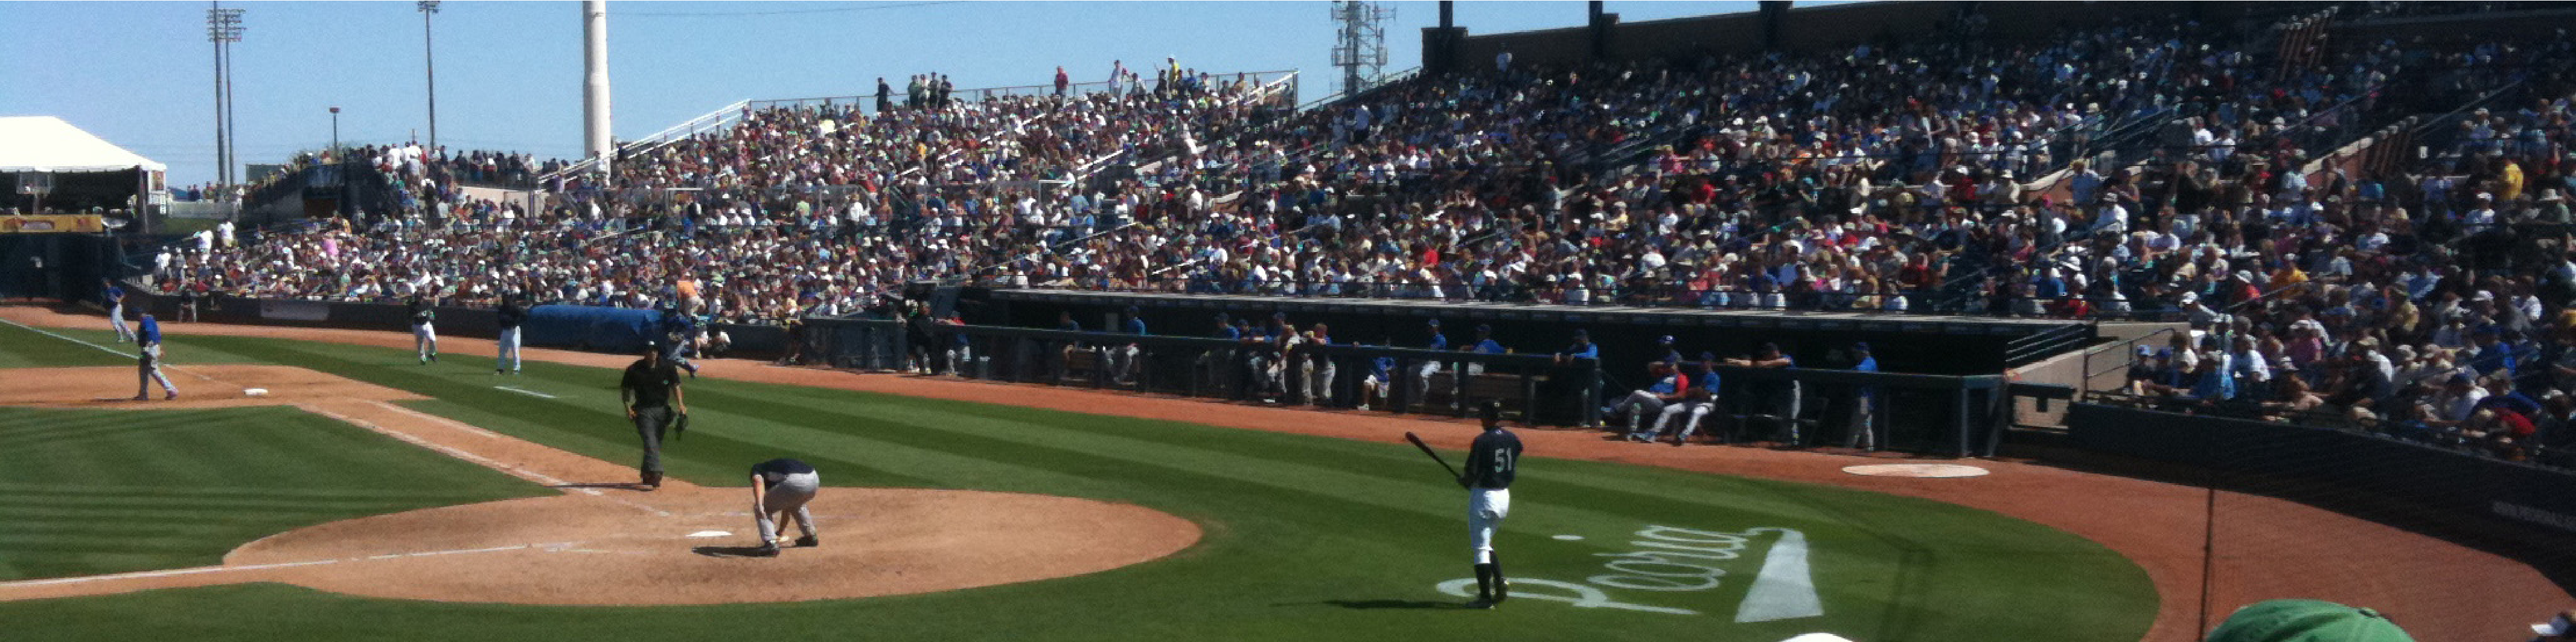
\includegraphics[width=\textwidth]{sampleteaser}
%   \caption{Seattle Mariners at Spring Training, 2010.}
%   \Description{Enjoying the baseball game from the third-base
%   seats. Ichiro Suzuki preparing to bat.}
%   \label{fig:teaser}
% \end{teaserfigure}

% \begin{teaserfigure}
%   \centering
%   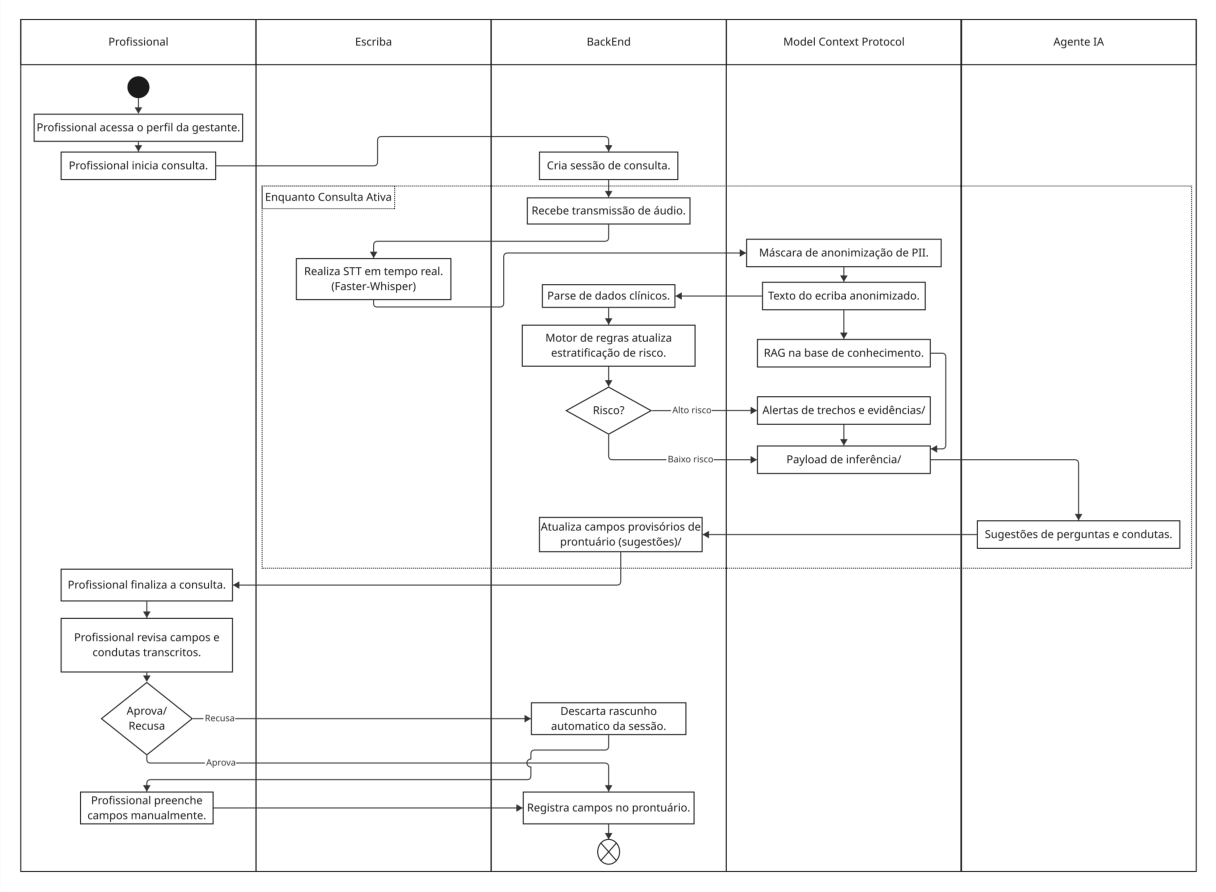
\includegraphics[width=\textwidth]{assets/FluxoDeConsulta.pdf}
%   \caption{Visão geral da arquitetura proposta para apoio documental e informacional no pré-natal, integrando transcrição local, mascaramento de dados sensíveis, recuperação aumentada por documentos oficiais, inferência local por LLM e validação humana obrigatória.}
%   \Description{Diagrama de arquitetura mostrando o fluxo entre profissional de saúde, transcrição local, gateway de privacidade, módulo RAG, LLM local e revisão humana.}
%   \label{fig:teaser}
% \end{teaserfigure}

%%
%% This command processes the author and affiliation and title
%% information and builds the first part of the formatted document.
\maketitle

\section{Introdução}
\label{sec:intro}
A Inteligência Artificial (IA) tem demonstrado potencial transformador na saúde pública, oferecendo soluções para otimização de fluxos de trabalho e suporte à decisão \cite{Rajpurkar2022, Cabitza2022, zuin2022prediction, zuin2025community}.
No contexto do atendimento pré-natal, estudos com bases reais de imagem e avaliação fetal têm explorado análises clínicas específicas, como a avaliação de expressões faciais associadas à dor fetal \cite{Rosa2020FetalPain, Bernardes2022FetalPain}, reforçando o interesse em soluções digitais aplicadas ao acompanhamento pré-natal.
Contudo, a mortalidade e a morbidade materna no Brasil permanecem como desafios persistentes de saúde pública, associados a desigualdades no acesso à assistência pré-natal e à necessidade de correção dos dados oficiais sobre mortes maternas \cite{AcessoPreNatal2018, Laurenti2010}.

A documentação clínica no \textit{Sistema Único de Saúde} (SUS) combina registros em sistemas digitais e instrumentos físicos independentes, como fichas de pré-natal e a Caderneta da Gestante \cite{FichaPreNatal2018, CadernetaGestante2024}. Essa fragmentação dificulta a integração entre sistemas médicos~\cite{cifuentes2015electronic, kruse2016challenges}. Na prática clínica, a dispersão das informações também aumenta o esforço de documentação dos profissionais de saúde~\cite{moy2021measurement, moy2023understanding}, especialmente em contextos que exigem monitoramento contínuo, identificação de sinais de risco e consulta frequente a protocolos assistenciais. 

Essa demanda torna-se particularmente relevante no pré-natal de alto risco. Segundo as diretrizes dos Manuais de Gestação de Alto Risco do Ministério da Saúde \cite{ManualAltoRisco2022, ManualAltoRisco2012}, condições de risco ou morbidades pré-existentes exigem estratificação contínua e acesso rápido a protocolos de acompanhamento. Diante do volume de informações envolvido nesse processo, modelos generativos têm sido propostos como assistentes virtuais clínicos para resumo e triagem de dados \cite{Clusmann2023, Rajpurkar2022}.

No entanto, a implantação irrestrita de Modelos de Linguagem de Grande Escala (LLMs) em cenários públicos de saúde enfrenta barreiras críticas, incluindo o risco de exposição de dados sensíveis (\textit{Personally Identifiable Information} -- PII), com potenciais implicações para a conformidade com a Lei Geral de Proteção de Dados (LGPD) \cite{OWASPLLM2025, LGPD2018}. Além disso, estudos apontam limitações no uso autônomo desses modelos em decisões clínicas, incluindo falhas em seguir instruções e sensibilidade ao contexto fornecido~\cite{hager2024evaluation}, bem como risco de geração de respostas não fundamentadas ou clinicamente inadequadas~\cite{asgari2025framework}.

Diante dessas limitações, este trabalho propõe a especificação, implementação e avaliação de uma plataforma digital \textit{on-premise} para apoio documental ao pré-natal, com foco no registro clínico durante a própria consulta, sem substituir a validação profissional. A abordagem proposta combina transcrição de voz para texto (\textit{Speech-to-Text}), recuperação aumentada (RAG) por documentos oficiais do Ministério da Saúde, mascaramento de PII, e validação profissional obrigatória. O trabalho também avalia em que medida modelos menores, executados localmente, podem alcançar desempenho próximo ao de modelos fechados de maior porte nessa tarefa, dentro de limites computacionais razoáveis para uso cotidiano. Essa comparação é relevante porque pode reduzir a dependência de serviços externos no processamento de áudio e dados textuais sensíveis. 

Embora a adoção de RAG busque aproximar as respostas dos protocolos utilizados como base documental, ela não elimina a necessidade de avaliar a aderência das saídas geradas. Da mesma forma, o mascaramento de PII antes da inferência reduz a exposição de dados sensíveis, mas não substitui mecanismos de validação e controle ao longo do fluxo. Por isso, a arquitetura proposta é concebida como um sistema assistivo e não autônomo, no qual o modelo generativo não recebe autonomia decisória nem persiste informações sem validação profissional. A partir dessa delimitação, este trabalho baseia-se na seguinte pergunta norteadora: \textit{Como especificar, implementar e avaliar um protótipo on-premise para apoio documental ao pré-natal a partir de protocolos públicos, sem atribuir autonomia decisória ao modelo generativo?}
Essa pergunta norteadora desdobra-se nas seguintes questões de pesquisa, identificadas como RQ1--RQ5 ao longo do artigo:
\begin{itemize}
\item \textbf{RQ1:} Como estruturar uma arquitetura local em contêineres que reduza o risco de exposição de áudio ou dados textuais sensíveis?
  \item \textbf{RQ2:} Qual é o desempenho do módulo RAG na recuperação de documentos e trechos relevantes dos manuais oficiais de pré-natal?
	\item \textbf{RQ3:} Qual é a aderência das respostas geradas por um LLM local aos protocolos de atendimento pré-natal no SUS?
	\item \textbf{RQ4:} Em que medida um anonimizador de dados pessoais sensíveis mascara entidades antes da inferência pelo modelo generativo?
	\item \textbf{RQ5:} Quais são os custos de latência associados à execução local em comparação com uma linha de base externa?
\end{itemize}


O objetivo geral deste trabalho é especificar, implementar e avaliar uma plataforma digital \textit{on-premise} para apoio documental ao pré-natal, integrando um \textit{LLM} fundamentado por \textit{RAG} e mecanismos de mascaramento de PII, com ênfase em explicabilidade, privacidade por desenho, auditabilidade e alinhamento às diretrizes públicas de saúde. Para atingir esse objetivo, delineiam-se os seguintes objetivos específicos:

\begin{enumerate}
  \item Desenvolver um protótipo funcional voltado à consulta assistida de informações de pré-natal, mantendo revisão humana obrigatória;
  \item Implementar um módulo de anonimização dedicado ao mascaramento e sanitização de PII brasileiras;
  \item Estruturar a recuperação de conhecimento com base em documentos públicos oficiais;
  \item Avaliar o desempenho do protótipo por meio de métricas de recuperação, aderência automática de respostas em testes sintéticos e análise de latência.
  \item Analisar os ganhos e perdas entre privacidade local, custo computacional, latência e viabilidade de implantação em ambientes de produção.
\end{enumerate}

O artigo está organizado da seguinte forma: a Seção~\ref{sec:ref} apresenta os fundamentos teóricos que orientam a proposta; as Seções~\ref{sec:materiais} e~\ref{sec:metodo} descrevem os materiais, o ambiente experimental, a arquitetura e as interfaces da plataforma; e a Seção~\ref{sec:avaliacao} apresenta os experimentos conduzidos para responder às perguntas de pesquisa. Por fim, a Seção~\ref{sec:discussao} discute os resultados obtidos, e a Seção~\ref{sec:conc} sintetiza as conclusões do estudo.


%Portanto, a justificativa técnica deste projeto fundamenta-se na estruturação de uma arquitetura local e auditável para apoio documental ao pré-natal, reduzindo a dependência de serviços externos no processamento de áudio e texto sensível. A proposta combina execução \textit{on-premise}, recuperação aumentada por documentos oficiais do Ministério da Saúde e revisão humana obrigatória, de modo que o modelo generativo não receba autonomia decisória nem persista informações sem validação profissional.

%A adoção de RAG busca reduzir o risco de respostas desvinculadas dos protocolos utilizados como base documental, embora não elimine a necessidade de avaliação de aderência e de revisão humana.
%De forma complementar, o gateway de privacidade aplica mecanismos de detecção e mascaramento de PII antes da inferência pelo modelo generativo, contribuindo para um fluxo mais controlável sob a perspectiva de privacidade por desenho, minimização de dados e auditabilidade.
%Assim, o foco do trabalho não é demonstrar eficácia assistencial, mas avaliar a viabilidade técnica, os limites e os trade-offs de uma arquitetura assistiva, local e não autônoma para o contexto do SUS.

%A pesquisa baseia-se na seguinte pergunta norteadora: \textit{Como especificar, implementar e avaliar um protótipo 'on-premise' para apoio documental ao pré-natal a partir de protocolos públicos, sem atribuir autonomia decisória ao modelo generativo?}

%O restante deste artigo está estruturado da seguinte forma: o referencial teórico embasa as decisões de design; os materiais e a metodologia detalham o ambiente e o fluxo de desenvolvimento; a solução proposta apresenta a arquitetura e interfaces criadas; e as seções finais discutem o desempenho e as limitações do ecossistema.


\section{Referencial Teórico}
\label{sec:ref}
%Esta seção define os conceitos centrais do trabalho e indica como cada um responde a riscos do uso de LLMs no pré-natal do SUS.
%\subsection{IA Responsável e Governança Clínica}

Sistemas de IA aplicados a contextos clínicos exigem mecanismos explícitos de supervisão, responsabilização e controle de uso. Em abordagens centradas no humano, a automação deve preservar a agência do profissional, tornar suas limitações visíveis e evitar que recomendações algorítmicas sejam incorporadas ao fluxo assistencial sem revisão adequada \cite{Shneiderman2021, Cabitza2022}. Esses princípios são particularmente relevantes para sistemas generativos, que podem ocultar incertezas, omissões ou inconsistências na resposta produzida.

Modelos de Linguagem de Grande Escala baseados apenas em conhecimento paramétrico têm limitações para recuperar informações atualizadas, indicar a origem de uma afirmação e manter aderência a documentos normativos específicos~\cite{mallen2023not}. A técnica de \textit{Retrieval-Augmented Generation} (RAG) aborda parte desse problema ao recuperar evidências externas em tempo de inferência e condicionar a geração textual ao contexto documental recuperado \cite{Lewis2020RAG}. Em saúde e biomedicina, revisões recentes indicam que RAG pode melhorar a fundamentação factual das respostas, mas sua eficácia depende da qualidade da recuperação, da fidelidade ao contexto, da robustez frente a ruído documental, da latência e dos critérios utilizados para avaliar as saídas geradas \cite{amugongo2025retrieval, Sharma2025RAGSurvey}.

O uso de RAG em bases normativas e diretrizes clínicas aproxima modelos generativos de fontes documentais controladas, o que é relevante em tarefas nas quais a resposta deve estar vinculada a protocolos específicos. Estudos aplicados a protocolos e diretrizes médicas sugerem que a recuperação de trechos normativos pode apoiar a consistência das respostas, desde que o corpus, a indexação e os critérios de avaliação sejam adequados ao domínio \cite{ke2025retrieval}. De forma relacionada, trabalhos recentes também têm avaliado RAG em cenários clínicos com modelos localmente implantáveis. Wada et al.~\cite{wada2025radiology}, por exemplo, avaliam um modelo Llama executado localmente com RAG em uma tarefa de consulta sobre contraste radiológico, comparando seu desempenho com modelos fechados acessados em nuvem. Outros trabalhos aproximam o RAG de tarefas clínicas complementares. Wo{\l}k~\cite{wolk2025evaluating} avalia variantes de RAG para apoio à decisão clínica em implantação on-premises, enquanto Lopez et al.~\cite{lopez2025clinical} propõem um pipeline de recuperação aumentada por entidades clínicas para extração de informações em notas clínicas.


A contribuição deste trabalho, porém, não se limita a avaliar se um modelo local com RAG responde adequadamente a uma consulta clínica especializada. O foco está em integrar esse tipo de modelo a um fluxo documental de pré-natal no SUS, no qual a resposta gerada é apenas uma etapa intermediária entre a recuperação de evidências oficiais, o preenchimento provisório de campos clínicos e a validação profissional antes da persistência no prontuário. Essa diferença é relevante porque desloca a avaliação de um cenário de pergunta e resposta para uma arquitetura assistiva com controle de privacidade, rastreabilidade documental e separação explícita entre sugestão algorítmica, decisão profissional e registro final.

Essa separação é necessária porque métricas automáticas isoladas não asseguram, por si só, a segurança, a utilidade e a adequação clínica das respostas geradas por LLMs em saúde \cite{tam2024framework}. Em sistemas de apoio documental, uma resposta formalmente plausível pode ainda estar incompleta, fora de contexto ou inadequada para incorporação ao registro clínico. Por isso, a revisão profissional obrigatória é tratada como requisito de segurança e de delimitação da autonomia do sistema, não apenas como etapa de interface.

Além dos desafios de aderência clínica, a integração de LLMs a fluxos assistenciais amplia riscos de segurança e privacidade. O \textit{OWASP Top 10 for Large Language Model Applications} mapeia ameaças como injeção de \textit{prompt}, vazamento de dados sensíveis e manipulação de conteúdos recuperados por aplicações baseadas em LLMs \cite{OWASPLLM2025}. Revisões sobre privacidade em LLMs também destacam riscos de exposição, memorização ou reprodução de dados sensíveis, especialmente em domínios como saúde \cite{yao2024survey, chen2025survey}. Esses riscos tornam relevantes estratégias de minimização de dados antes da inferência, incluindo detecção e mascaramento de informações pessoalmente identificáveis.

\begin{table*}[tttt]
\centering
\caption{Dimensões exploradas por estudos relacionados.}
\label{tab:trabalhos_relacionados}
\small
\setlength{\tabcolsep}{3.5pt}
\renewcommand{\arraystretch}{1.18}

\begin{tabular}{p{1.8cm} p{3cm} p{3cm} c c c c c}
\toprule
\textbf{Referência}
& \textbf{Escopo}
& \textbf{Saída do modelo}
& \textbf{RAG}
& \begin{tabular}{@{}c@{}}\textbf{Execução}\\\textbf{local}\end{tabular}
& \begin{tabular}{@{}c@{}}\textbf{Corpus}\\\textbf{normativo}\end{tabular}
& \begin{tabular}{@{}c@{}}\textbf{Mascaramento}\\\textbf{de PII}\end{tabular}
& \begin{tabular}{@{}c@{}}\textbf{Persistência}\\\textbf{validada no registro}\end{tabular} \\
\midrule

Ke et al.~\cite{ke2025retrieval}
& Diretrizes clínicas pré-operatórias
& Resposta a consulta baseada em diretrizes
& \checkmark
& Parcial
& \checkmark
& Não avaliado
& Não avaliado \\

Wada et al.~\cite{wada2025radiology}
& Consulta sobre contraste radiológico
& Resposta clínica especializada
& \checkmark
& \checkmark
& Parcial
& Não avaliado
& Não avaliado \\

Lopez et al.~\cite{lopez2025clinical}
& Extração de informações em notas clínicas
& Variáveis clínicas extraídas de registros textuais
& \checkmark
& Não avaliado
& Não avaliado
& Não avaliado
& Não avaliado \\

Wo{\l}k~\cite{wolk2025evaluating}
& Apoio à decisão clínica com RAG on-premises
& Resposta de apoio à decisão baseada em vinhetas clínicas
& \checkmark
& \checkmark
& Parcial
& Não avaliado
& Não avaliado \\

Este trabalho
& Apoio documental ao pré-natal no SUS
& Sugestão provisória vinculada ao registro
& \checkmark
& \checkmark
& \checkmark
& \checkmark
& \checkmark \\

\bottomrule
\end{tabular}

\vspace{0.1cm}
\begin{minipage}{0.98\textwidth}
\scriptsize
\textit{Nota:} ``Não avaliado'' indica que a dimensão não aparece como eixo de avaliação ou contribuição principal no estudo citado e não implica ausência absoluta de discussão sobre o tema. No caso de privacidade, a tabela distingue discussões gerais sobre implantação local, dados desidentificados ou segurança operacional de mecanismos específicos de mascaramento de PII antes da inferência. ``Parcial'' indica que a dimensão aparece de forma relacionada, mas não como tema central ou com o mesmo escopo operacional adotado neste trabalho.
\end{minipage}
\end{table*}

A Tabela~\ref{tab:trabalhos_relacionados} sintetiza esse posicionamento em relação aos estudos mais próximos. Em conjunto, esses trabalhos mostram avanços importantes em RAG clínico, execução local, diretrizes médicas, extração de informações clínicas e mitigação de alucinações. Contudo, não tratam esses elementos como partes de um mesmo fluxo documental assistivo. Este trabalho se insere nessa lacuna ao articular documentos oficiais brasileiros, modelos locais, mascaramento de PII e validação profissional obrigatória em uma arquitetura voltada ao apoio documental ao pré-natal no SUS.

%Com base em princípios de IA responsável e design centrado no humano \cite{Shneiderman2021, Cabitza2022}, este trabalho adota mecanismos de transparência, responsabilização e supervisão humana como requisitos de projeto. No contexto proposto, esses princípios são operacionalizados por meio de uma arquitetura local (\textit{on-premise}), interfaces de revisão obrigatória das saídas do modelo e restrição explícita de autonomia decisória da IA.

%Modelos de Linguagem de Grande Escala baseados apenas em conhecimento paramétrico apresentam limitações para acessar, atualizar e prover proveniência sobre informações factuais. A técnica de \textit{Retrieval-Augmented Generation} combina geração textual com recuperação de evidências externas em tempo de inferência, condicionando a resposta ao contexto documental recuperado \cite{Lewis2020RAG}. Revisões recentes também apontam que a qualidade da recuperação, a fidelidade ao contexto e a robustez contra ruído permanecem desafios centrais em sistemas RAG \cite{Sharma2025RAGSurvey}. Aplicando essa premissa à arquitetura, o modelo foi ancorado exclusivamente em cartilhas e manuais oficiais do Ministério da Saúde, empregando particionamento (\textit{chunking}) semântico e hiperparâmetros conservadores para priorizar aderência documental em detrimento da fluidez generativa.

%No tocante à supervisão, a literatura de IA responsável centrada no humano defende que sistemas automatizados em domínios críticos devem preservar a agência humana e manter mecanismos claros de responsabilização \cite{Shneiderman2021}. Em consonância com essa diretriz, a plataforma adota estritamente a restrição \textit{human-in-the-loop}, na qual nenhuma predição, sugestão ou extração da Inteligência Artificial é salva de forma autônoma. O sistema atua como ferramenta assistiva e documental, exigindo que o médico ou enfermeiro valide ou edite os dados antes de sua persistência no prontuário eletrônico.

%A integração de LLMs em fluxos clínicos expande a superfície de ataques, demandando proteções contra injeção de \textit{prompt} e exposição de dados sensíveis, conforme mapeado pelo \textit{OWASP Top 10 for Large Language Model Applications} \cite{OWASPLLM2025}. Para endereçar essas vulnerabilidades regulatórias e técnicas, o ecossistema proposto incorpora um \textit{gateway} de privacidade customizado, munido de Expressões Regulares (RegEx) e Reconhecimento de Entidades Nomeadas (NER) operando localmente. Esse mecanismo atua higienizando identificadores de saúde brasileiros, como CPF e CNS, antes do trânsito de dados para o modelo, reduzindo o risco de vazamento de informações pessoalmente identificáveis.


\section{Materiais}
\label{sec:materiais}


Nesta seção, são detalhados os componentes que estruturam o sistema, incluindo os requisitos de \textit{hardware} para execução local, os \textit{frameworks} de desenvolvimento, as bases de dados utilizadas e as ferramentas de Inteligência Artificial implementadas.
%\subsection{Hardware}
A escolha do modelo obedeceu ao critério de viabilidade operacional local, sendo o protótipo executado em ambiente com CPU Intel i7-14700K, 32GB de RAM e GPU Nvidia RTX 5060 Ti com 16GB de VRAM.
Embora o model card do Qwen3.5 9B indique suporte a contexto padrão de 262.144 tokens, adotou-se uma janela operacional reduzida de 16.384 tokens no protótipo, em função das restrições locais de VRAM, latência e estabilidade de inferência \cite{Qwen35ModelCard2026}.
A escolha do Qwen3.5 9B quantizado em Q4 decorreu da compatibilidade com a VRAM disponível, evitando \textit{offloading} para RAM/CPU e aumento expressivo do tempo até o primeiro token (TTFT).

%\subsection{Software e Frameworks}
O ambiente adota \textit{TypeScript} como linguagem principal.
O \textit{backend} foi desenvolvido em \textit{Node.js} utilizando o micro-\textit{framework} Hono e o \textit{frontend} foi estruturado em React, empregando Vite e TailwindCSS.
A execução em contêineres \textit{Docker} contribui para segmentação lógica e isolamento operacional, reduzindo a exposição de PII em caso de comprometimento.
Para transcrição, integra-se o \textit{Faster-Whisper} com processamento local e descarte imediato do stream de áudio, evitando o envio a terceiros e reduzindo a superfície de vazamento.

A orquestração do LLM clínico ocorre via \textit{Ollama}; para apoio à decisão, empregam-se hiperparâmetros conservadores (Tabela~\ref{tab:hyperparams}) para reduzir a variabilidade, favorecendo a aderência ao contexto recuperado.

\begin{table}[h!]
  \centering
  \caption{Hiperparâmetros de inferência (Ollama) e RAG.}
  \label{tab:hyperparams}
  \small
  \begin{tabular}{l r | l r}
    \toprule
    \multicolumn{2}{c}{\textbf{LLM (Qwen3.5)}} & \multicolumn{2}{c}{\textbf{RAG \& Chunking}} \\
    \midrule
    \texttt{num\_ctx}                          & 16.384 & \texttt{embedding\_model}  & nomic-embed-text \\
    \texttt{num\_batch}                        & 256    & \texttt{chunk\_max\_chars} & 900              \\
    \texttt{temperature}                       & 0.1    & \texttt{max\_chunks}       & 6                \\
    \texttt{top\_p}                            & 0.9    & \texttt{rerank\_enabled}   & True             \\
    \bottomrule
  \end{tabular}
\end{table}

\subsection{Base de Dados}

A camada transacional (cadastros e triagens) utiliza \textit{PostgreSQL}, gerenciado via \textit{Prisma ORM}. 
As Cartilhas de Atenção Pré-Natal do Ministério da Saúde foram vetorizadas como fonte documental de referência (Tabela~\ref{tab:cartilhas_sus}).
O acervo inclui edições de 2010--2025 e para mitigar conflitos no RAG, cada documento foi associado a metadados de ano e origem, permitindo rastreabilidade das respostas geradas.

\begin{table}[b!]
  \centering
  \caption{Base de conhecimento documental: Manuais e cartilhas.}
  \label{tab:cartilhas_sus}
  %\footnotesize
  \begin{tabular}{l c c}
    \toprule
        \textbf{Título do Documento} & \textbf{Ano} & \textbf{Referência} \\ 
    \midrule
        Guia do Pré-natal do Parceiro [...]     & 2025 & \cite{GuiaPreNatalParceiro2025} \\
        Caderneta da Gestante                   & 2024 & \cite{CadernetaGestante2024} \\
        Guia de Atenção à Saúde                 & 2024 & \cite{GuiaAtencaoGestanteMG2024} \\
        Manual de Gestação de Alto Risco        & 2022 & \cite{ManualAltoRisco2022} \\
        Ficha Pré-natal                         & 2018 & \cite{FichaPreNatal2018} \\
        Atualização em Pré-natal [...]          & 2014 & \cite{AtualizacaoPreNatalSC2014} \\
        Cadernos de Atenção Básica              & 2012 & \cite{CadernosAtencaoBasica32} \\
        Manual Técnico Gestação de Alto Risco   & 2012 & \cite{ManualAltoRisco2012} \\
        Gestação de Alto Risco                  & 2010 & \cite{ManualAltoRisco2010} \\
    \bottomrule
  \end{tabular}
\end{table}

\subsection{Ferramentas de IA}

A seleção do modelo obedeceu a um critério de viabilidade operacional \textit{on-premise}, com 16GB de VRAM dedicados e janela de contexto configurada em 16.384 \textit{tokens} para RAG.
Modelos cujo consumo estimado de VRAM superasse 13GB após quantização Q4 foram descartados para evitar \textit{offloading} de memória, reconhecendo-se que essas estimativas são teóricas e dependem da arquitetura de hardware, \textit{drivers}, mecanismo de inferência e parâmetros de execução \cite{VRAMCalculator}.

\begin{table}[t!]
  \centering
  \begin{threeparttable}
  \caption{Estimativa teórica de consumo de VRAM.}
  \label{tab:latency_compatibility}
  %\footnotesize
  \begin{tabular}{l c c r}
    \toprule
    \textbf{Modelo}       & \textbf{Contexto} & \textbf{Parâmetros} & \textbf{VRAM}           \\
    \midrule
    Qwen3.6 (Q4)          & 16.384            & 35B                 & $\sim$24 GB             \\
    Qwen3.5 (Q4)          & 16.384            & 27B                 & $\sim$27.4 GB           \\
    GPT-OSS (Q4)          & 16.384            & 20B                 & $\sim$17.3 GB           \\
    Qwen3 (Q4)            & 16.384            & 14B                 & $\sim$16.12 GB          \\
    \textbf{Qwen3.5 (Q4)} & \textbf{16.384}   & \textbf{9B}         & \textbf{$\sim$10.51 GB} \\
    Qwen3 (Q4)            & 16.384            & 8B                  & $\sim$10.41 GB          \\
    \bottomrule
  \end{tabular}
  \begin{tablenotes}
    \footnotesize
    \item[*] Cálculo de VRAM teórico estimado baseado em https://apxml.com/tools/vram-calculator.
  \end{tablenotes}
  \end{threeparttable}
\end{table}

Para a escolha entre os candidatos compatíveis com 16GB de VRAM sem \textit{offloading} de memória, dentre o conjunto de candidatos, o Qwen3.5 9B foi considerado para combinar menor demanda de memória com uma geração mais recente da família Qwen, cujo \textit{model card} informa suporte a contexto nativo de 262.144 tokens \cite{Qwen35ModelCard2026}.
Para complementar o critério de escolha, consultou-se o comparativo público não revisado por pares LLMBase \cite{benchmarks_llm}. Embora esses resultados não reproduzam a arquitetura local deste trabalho, o comparativo indica vantagem do Qwen3.5 9B sobre o Qwen3 14B em métricas como GPQA (80,6\% contra 60,4\%) e índice composto de inteligência (32,4 contra 16,2).

A inferência é orquestrada pelo \textit{Ollama} com o modelo Qwen3.5 (9B, quantização Q4) da Alibaba, parametrizado para mitigar alucinações 
%(Tabela~\ref{tab:hyperparams}) 
(Tabela~\ref{tab:latency_compatibility}) na arquitetura de hardware disponível.
A estruturação da base de conhecimento inclui o particionamento semântico (\textit{chunking}) das diretrizes e sua vetorização única, com persistência no armazenamento vetorial.

Na etapa de recuperação, adotou-se \textit{Maximal Marginal Relevance} (MMR) como estratégia de reranqueamento/diversificação dos trechos recuperados.
O MMR seleciona iterativamente os \textit{chunks} que apresentam alta similaridade com a consulta, mas penaliza trechos muito semelhantes aos já escolhidos, buscando equilibrar relevância e diversidade no contexto enviado ao modelo \cite{CarbonellGoldstein1998MMR}.
Essa técnica foi utilizada para reduzir redundância no contexto recuperado, não como mecanismo isolado de resolução de divergências entre edições distintas dos manuais.



\section{Metodologia}
\label{sec:metodo}
A pesquisa adota a Engenharia de Software com desenvolvimento ágil (Scrum) para construção do artefato, organizada em cinco frentes integradas:
(i) modelagem relacional do prontuário;
(ii) \textit{WebApp} de gestão e consulta de pacientes;
(iii) agente escriba do tipo \textit{overhearing}, contemplando transcrição autorizada da consulta em andamento e sugestão de preenchimentos e condutas sem necessidade de interação explícita;
(iv) motor RAG ancorado nas cartilhas do Ministério da Saúde;
e (v) assistente local de consulta contextual, operado via chat, voltado a responder perguntas explícitas com base no contexto do prontuário e documentos recuperados.

A arquitetura reflete o isolamento dos módulos em três subredes \textit{Docker} (\texttt{frontend-nw}, \texttt{backend-nw} e \texttt{data-nw}), conforme a \textit{stack} detalhada na Seção 3 (Materiais). 

A sanitização de PII e a adoção do modo \textit{zero-trust} seguem o módulo de privacidade descrito anteriormente, fundamentando-se nos requisitos de minimização da LGPD apresentados na Seção 2.
Todo o áudio capturado é processado localmente e descartado ao final da interação.

A Figura~\ref{fig:fluxo_consulta} sintetiza o ciclo de vida da transação da consulta médica, estruturado nas seguintes etapas operacionais:

% \begin{figure}[htbp]
%   \centering
%   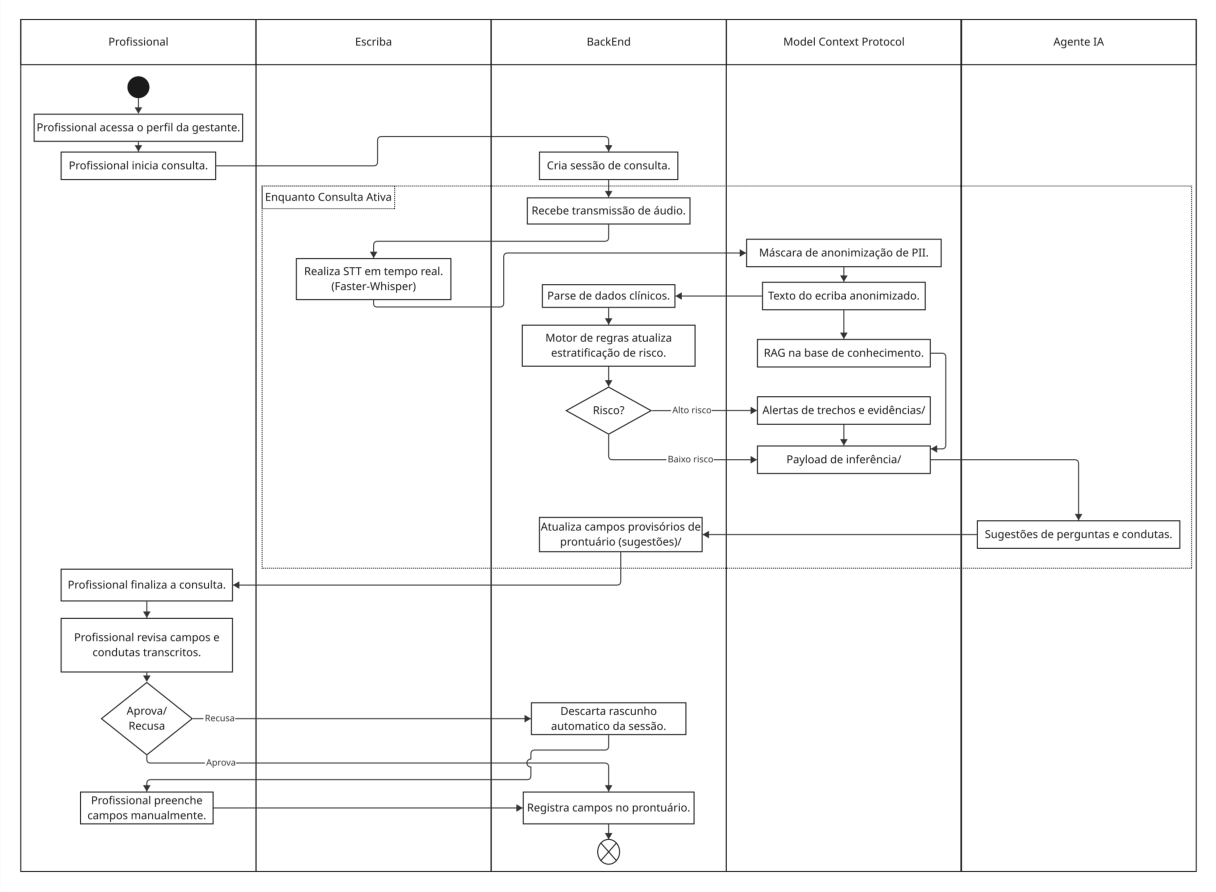
\includegraphics[width=\textwidth, keepaspectratio]{assets/FluxoDeConsulta.pdf}
%   \caption{Pipeline arquitetural e ciclo de vida da transação da consulta médica.}
%   \label{fig:fluxo_consulta}
% \end{figure}

\begin{figure*}[htbp]
  \centering
  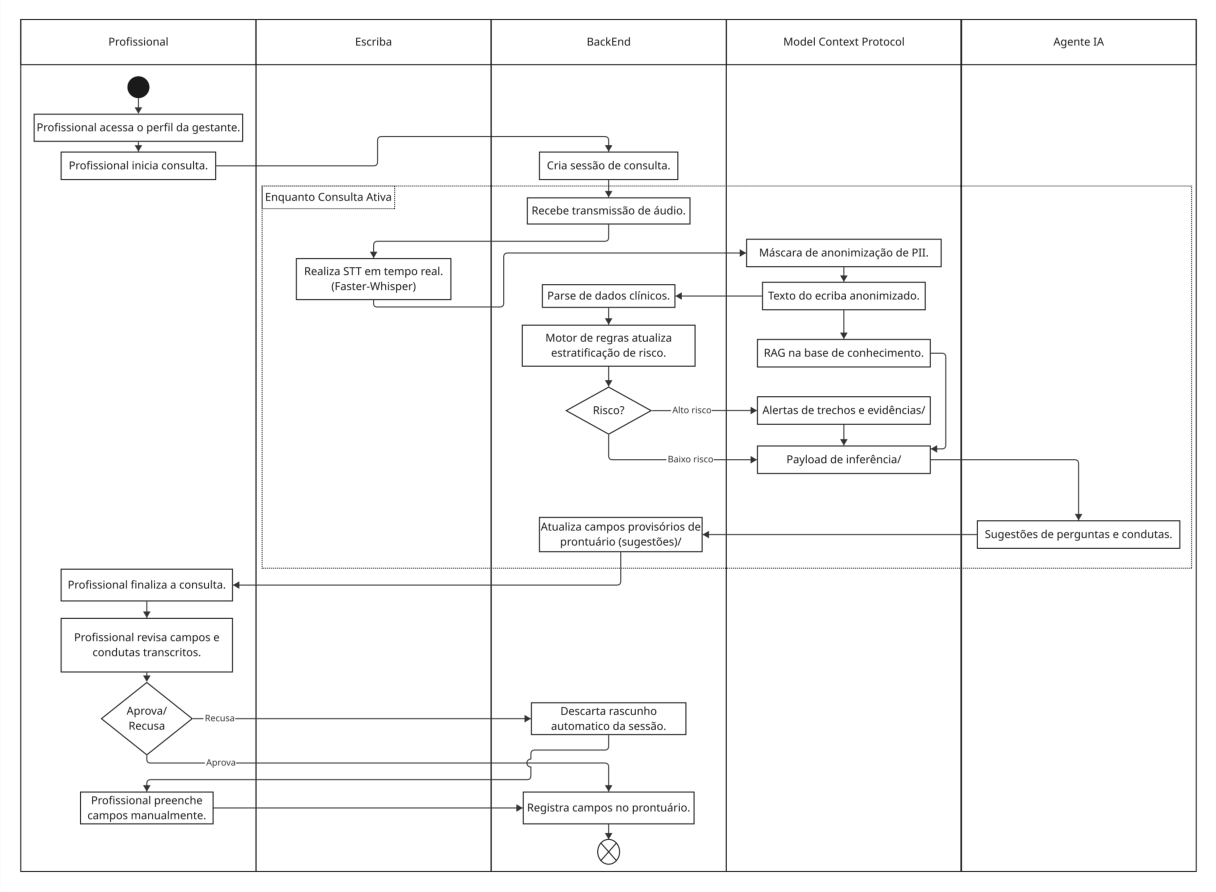
\includegraphics[width=0.8\textwidth]{assets/FluxoDeConsulta.pdf}
  \caption{Pipeline arquitetural e ciclo de vida da transação da consulta médica.}
  \label{fig:fluxo_consulta}
\end{figure*}

\begin{itemize}
  \item \textbf{Captura e transcrição local (STT):} o fluxo de áudio é transcrito em tempo de execução via \textit{Whisper} com diarização.
  \item \textbf{Sanitização de entrada:} o \textit{gateway} remove ou mascara as \textit{PII} na transcrição antes de compor a consulta ao módulo RAG.
  \item \textbf{Recuperação (Retriever):} a busca retorna os trechos relevantes e aplica MMR para diversificar os \textit{chunks} selecionados e reduzir redundâncias no contexto enviado ao modelo.
  \item \textbf{Geração (Generator):} o LLM sintetiza a resposta clínica com hiperparâmetros conservadores, privilegiando a aderência ao contexto recuperado.
  \item \textbf{Apresentação e validação humana:} a interface exibe as sugestões de preenchimento, mantendo a edição manual integralmente disponível.
\end{itemize}

Para cumprir a restrição de segurança clínica, adota-se uma abordagem baseada no conceito de \textit{Human-in-the-Loop}, onde nenhum dado sugerido pela IA é gravado no banco de dados sem a confirmação explícita do profissional (US04), garantindo o controle total sobre o registro.
A principal ameaça à validade interna é a geração de conteúdo não evidenciado nos protocolos da base de conhecimento, sendo esta mitigada por RAG restrito às diretrizes oficiais e \textit{Human-in-the-Loop}.

A ameaça de exposição de \textit{PII} é mitigada por processamento local em um \textit{gateway} de mascaramento aplicado antes da recuperação e inferência.
O anonimizador foi implementado em arquitetura híbrida, combinando regras determinísticas de Expressões Regulares (RegEx) para identificadores brasileiros e um módulo de Reconhecimento de Entidades Nomeadas (NER) especializado em português biomédico.
Como modelo de NER, utilizou-se o\linebreak \texttt{OpenMed-PII-Portuguese-SnowflakeMed-Large-568M-v1}~\cite{openmed-pii-2026}.%, disponibilizado no Hugging Face \cite{openmed-pii-2026}.

A modelagem relacional foi derivada da 8ª edição revisada da Caderneta da Gestante, contemplando entidades para paciente, gestação, consultas, sinais vitais, exames, antecedentes, prontuário e registros de atendimento.
O DER completo foi disponibilizado como material suplementar no repositório do projeto.

O módulo de transcrição baseado em Faster-Whisper foi integrado ao protótipo para validar a viabilidade técnica do fluxo de captura local de áudio. Contudo, sua avaliação sistemática não compõe o escopo experimental deste trabalho, permanecendo como etapa futura.

\subsection{Solução Proposta}
\label{sec:solucao}

A arquitetura derivou de requisitos funcionais (RF) e histórias de usuário (US) mapeados a riscos clínicos, operacionais e regulatórios.
A Tabela~\ref{tab:rf_riscos} resume essa relação, demonstrando como as ferramentas teóricas abordadas foram convertidas em funcionalidades práticas no protótipo.

\begin{table*}[htbp]
  \centering
  \caption{Requisitos, riscos mitigados e mecanismos de controle.}\label{tab:rf_riscos}
  %\scriptsize
  \makebox[\textwidth][c]{
    \begin{tabularx}{\textwidth}{l X X X}
      \toprule
      \textbf{RF/US}	& \textbf{Risco} 			& \textbf{Decisão de design} 			& \textbf{Mitigação esperada} \\
      \midrule
      RF03/04 		& Retenção indevida de áudio.     	& STT local; áudio não persistido. 		& Reduz superfície de vazamento. \\
      RF05  & Alucinação em conduta clínica. & RAG restrito a manuais; \textit{system prompts} com escopo limitado; \textit{guardrails} para recusa fora do contexto recuperado & Respostas embasadas em protocolo oficial. \\
      US04 	& Automação indevida. & Bloqueio de persistência sem aprovação; \textit{guardrails} para exigir validação humana & Decisão final sob responsabilidade do profissional. \\
      US13 		& Exposição de PII ao modelo. 		& \textit{Gateway} de anonimização. 		& Dados em trânsito anonimizados \\
      US05 		& Atraso na identificação de alto risco. & Alertas determinísticos por limiares das cartilhas. 		& Sinalização visual imediata na consulta \\
      US06 		& Descontinuidade do registro físico. 	& Exportação PDF. 				& Continuidade do cuidado manual \\
      \bottomrule
    \end{tabularx}
    }
  \end{table*}

As interfaces do protótipo de alta fidelidade, incluindo agenda de atendimentos, prontuário consolidado e tela de consulta ativa com o agente Escriba, foram disponibilizadas como material suplementar no repositório do projeto.


\section{Avaliação Experimental e Resultados}
\label{sec:avaliacao}
A avaliação experimental foi conduzida em três frentes complementares: recuperação documental, geração de respostas e segurança do fluxo clínico, associadas às RQ2, RQ3 e RQ4, respectivamente. A RQ1 é avaliada de forma complementar pelos testes funcionais de segurança do fluxo, enquanto a RQ5 é tratada na análise de latência. 
O objetivo foi verificar se a arquitetura proposta, baseada em RAG, LLM local e \textit{gateway} de privacidade, consegue recuperar evidências dos manuais oficiais, produzir respostas aderentes aos protocolos e impedir vazamento de informações sensíveis antes da inferência.
O conjunto de testes utilizado contém 100 perguntas em português, das quais 90 avaliam aderência a protocolos e 10 são perguntas distratoras (\textit{trap}).
A distribuição por dificuldade foi de 42 itens fáceis, 35 médios e 23 difíceis.
Os níveis de dificuldade foram definidos manualmente durante a construção do benchmark.
Questões fáceis correspondem a consultas diretas cuja resposta pode ser localizada em um único documento ou trecho protocolar.
Questões de dificuldade média exigem combinar múltiplas informações presentes em diferentes seções de um mesmo manual ou em documentos distintos.
Questões difíceis envolvem cenários menos frequentes, exceções protocolares ou situações que demandam maior especificidade terminológica para recuperação da evidência correta.
Quatro itens classificados como \texttt{human\_judge} foram mantidos para revisão qualitativa e não compõem o denominador da métrica automática de APR.
Este sistema de avaliação foi inspirado por práticas da indústria para avaliação de agentes de IA, como as avaliações de agentes do \textit{Microsoft Copilot Studio} \cite{MicrosoftCopilotEval2026}.

%--------------------------------------------------------------------------------------------

\subsection{Recuperação Semântica}

%O módulo de recuperação foi avaliado isoladamente com \textit{top-k}=6 e expansão de consulta ativada.
O módulo de recuperação, correspondente à RQ2, foi avaliado isoladamente com \textit{top-k}=6 e expansão de consulta ativada.
O valor de $k$ foi definido como escolha operacional intermediária, buscando equilibrar cobertura documental e controle de ruído no contexto enviado ao modelo.
Foram utilizadas três métricas:
\textit{Hit@6}, que verifica se o documento-fonte esperado aparece entre os seis primeiros \textit{chunks};
\textit{Mean Reciprocal Rank} (MRR), que mede quão cedo o primeiro documento correto aparece na lista recuperada. Quanto mais próximo da primeira posição estiver o documento esperado, maior será o valor da métrica, aproximando-se de 1;
e \textit{phrase\_recall}, que mede a presença das frases esperadas nos trechos recuperados.
Além de apoiar a geração de respostas, o RAG acrescenta uma camada de rastreabilidade documental ao sistema, pois permite associar cada resposta aos trechos recuperados, seus documentos de origem e respectivos metadados.
Essa característica aumenta a auditabilidade das respostas e favorece a revisão humana, aspecto relevante em sistemas de apoio informacional no contexto médico.
A Tabela~\ref{tab:metricas_rag} apresenta os resultados por dificuldade.

\begin{table}[t!]
  \centering
  \caption{Desempenho do módulo RAG por nível de dificuldade ($n=100$).}
  \label{tab:metricas_rag}
  %\small
  \begin{tabular}{lccc}
  	\toprule
  	\textbf{Dificuldade} & \textbf{n}   & \textbf{Hit@6 (\%)}  & \textbf{MRR Médio} \\
  	\midrule
  	Easy                 & 42           & 76,2\%               & 0,4837             \\
  	Medium               & 35           & 68,6\%               & 0,3633             \\
  	Hard                 & 23           & 95,7\%               & 0,6536             \\
  	\midrule
  	\textbf{Global}      & \textbf{100} & \textbf{78,0\%}      & \textbf{0,4807}    \\
  	\bottomrule
  	\end{tabular}
  \end{table}
  
O \textit{phrase\_recall} médio global foi de 47,1\%.
Embora os casos encontrados nos itens difíceis representem situações potencialmente mais complexas do ponto de vista clínico, eles frequentemente utilizam terminologia mais específica e menos ambígua, o que favorece a recuperação vetorial.
Em contraste, perguntas rotineiras de pré-natal apresentam maior sobreposição semântica entre documentos, aumentando a competição entre trechos similares durante o ranqueamento.

%--------------------------------------------------------------------------------------------

\subsection{Geração de Resposta}

A aderência das respostas aos protocolos, eixo da RQ3, foi avaliada por meio da Taxa de Aprovação de Respostas (APR) correspondente à proporção de frases obrigatórias aprovadas segundo os critérios de protocolo, calculada sobre itens elegíveis à avaliação automática, e da Taxa de Falha em Perguntas Distratoras (TFR), calculada sobre os itens \textit{trap}.
O modelo local Qwen3.5 9B foi executado com e sem RAG para medir o ganho incremental da recuperação.
O Gemini-3.1-Flash-Lite foi utilizado apenas como linha de base externa de comparação, recebendo o mesmo contexto recuperado pelo RAG do protótipo, mas sem integrar a arquitetura \textit{on-premise} proposta.

\begin{table}[h!]
  \centering
  \caption{Desempenho dos modelos na geração de respostas.}
  \label{tab:apr_tfr_providers}
  \small
  \begin{tabular}{lccc}
  	\toprule
  	\textbf{Provedor}           & \textbf{Modo RAG} & \textbf{APR (\%)} & \textbf{TFR (\%)} \\
  	\midrule
  	Qwen3.5 9B (Ollama)         & Off               & 53,1\% (51/96)    & 20,0\% (2/10)     \\
	  Qwen3.5 9B (Ollama)         & On                & 57,3\% (55/96)    & 10,0\% (1/10)     \\
  	Gemini-3.1-Flash-Lite       & On                & 61,5\% (59/96)    & 0\% (0/10)      \\
  	\bottomrule
  \end{tabular}
  \end{table}

A ativação do RAG no modelo local elevou a APR de 53,1\% para 57,3\% e reduziu a TFR de 20,0\% para 10,0\%.
O ganho é limitado, indicando que a recuperação documental contribui para reduzir respostas inseguras, mas não garante aderência clínica estrita quando o modelo precisa negar condutas, reproduzir termos literais ou resolver conflitos entre documentos.
No conjunto total de execuções, foram registradas 3 falhas em itens \textit{trap} e 120 reprovações de protocolo nas 258 avaliações automáticas de frases obrigatórias.
Os quatro itens excluídos da avaliação demandam revisão qualitativa da equipe clínica e não entram no denominador da Tabela~\ref{tab:apr_tfr_providers}.

%--------------------------------------------------------------------------------------------

\subsection{Privacidade, escopo e latência}

A avaliação do mascaramento de PII, correspondente à RQ4, submeteu o módulo de anonimização a 50 frases sintéticas, totalizando 76 entidades sensíveis avaliadas, incluindo CPF, Cartão Nacional de Saúde (CNS), e-mail, telefone, nomes completos e cadeias numéricas longas.
Não houve vazamento detectado no conjunto testado, conforme a Tabela~\ref{tab:pii_leak}. Esse resultado valida a implementação inicial do mascaramento, mas não elimina a necessidade de testes com variações linguísticas, abreviações e ruído de transcrição.

\begin{table}[b!]
  \centering
  \caption{Taxa de vazamento de PII por tipo de entidade.}
  \label{tab:pii_leak}
  %\small
  \begin{tabular}{lcc}
  	\toprule
	\textbf{Entidade} 	 	                & \textbf{n} 		                & \textbf{Leak Rate (\%)} \\
	\midrule
  	CNS     			                      & 11                            & 0\%                   \\
  	CPF                                 & 12                            & 0\%                   \\
  	E-mail                              & 12                            & 0\%                   \\
  	Nome Completo			                  & 21                            & 0\%                   \\
  	Cadeias Numéricas Longas            & 8                             & 0\%                   \\
  	Telefone                            & 12                            & 0\%                   \\
	\midrule
  	\textbf{Total Global}               & \textbf{76}                   & \textbf{0\%}          \\
  	\bottomrule
  \end{tabular}
  \end{table}

\begin{table*}[h!]
  \centering
  \caption{Latência média por configuração de execução.}
  \label{tab:latencia_config}
  %\small
  \begin{tabular}{lrrrr}
    \toprule
    \textbf{Configuração} 		& \textbf{Retrieve (ms)} 	& \textbf{Latência total (s)} 	& \textbf{TTFT (ms)} 	& \textbf{tokens/s} \\
    \midrule
    Qwen3.5 9B (Ollama)			& --    		 	& 11,71 			& 470,1  		& 32,5 \\
    Qwen3.5 9B (Ollama)   + RAG on  	& 373,1 			& 15,59 			& 2789,7 		& 32,4 \\
    Gemini-3.1-Flash-Lite + RAG on 	& 372,7 			& 4,55  			& 3501,9 		& 360,6 \\
    \bottomrule
  \end{tabular}
\end{table*}

Além das métricas agregadas, o roteiro funcional (GT01-GT05) avaliou aspectos operacionais ligados à RQ1, com cinco casos sintéticos voltados a comportamentos essenciais do protótipo. Os casos GT01, GT02 e GT03 avaliam respostas clínicas com RAG e LLM em cenários de risco alto extraídos dos manuais protocolares.
O GT04 avalia sanitização direta de PII.
O GT05 avalia a capacidade de recusar uma requisição fora do escopo de pré-natal.

O roteiro funcional obteve sucesso em quatro dos cinco casos avaliados.
Os três casos clínicos com RAG e LLM foram aprovados, assim como o caso de sanitização direta de PII.
A falha ocorreu no GT05, no qual a barreira de escopo não conteve adequadamente uma requisição fora do domínio pré-natal.
Esse resultado indica que a segurança comportamental não deve depender apenas de \textit{system prompts} e o módulo de privacidade deve incorporar verificações determinísticas ou classificadores de escopo antes da síntese pelo modelo.


A RQ5 foi analisada a partir das métricas de eficiência computacional, segregadas por configuração para evitar que a linha de base em nuvem distorça a interpretação operacional do modelo local.
%Quanto à eficiência computacional, as métricas foram segregadas por configuração para evitar que a linha de base em nuvem distorça a interpretação operacional do protótipo local.
A Tabela~\ref{tab:latencia_config} apresenta os resultados médios encontrados.

Para o protótipo local, a recuperação vetorial acrescentou aproximadamente 373 ms ao fluxo, enquanto a latência total do Qwen3.5 9B com RAG foi de 15590,1 ms.
Portanto, o gargalo operacional permanece na inferência local do LLM e no aumento de contexto provocado pelo RAG, não na busca vetorial.
A linha de base externa apresentou maior vazão de geração, mas não representa a premissa de privacidade local da arquitetura proposta.
Esse resultado reforça que a adoção em produção de baixo custo ainda é limitada pelos requisitos de hardware, especialmente VRAM, tempo de inferência e estabilidade sob carga.


\section{Discussão}
\label{sec:discussao}
Os resultados indicam viabilidade técnica parcial da arquitetura proposta.
A combinação de execução local, RAG restrito a documentos oficiais e mascaramento de PII atende ao objetivo de reduzir dependência de nuvem pública e de oferecer um fluxo mais controlável do ponto de vista da LGPD.
Os resultados mostram que o protótipo ainda não pode ser interpretado como sistema autônomo de apoio clínico, o protótipo foi concebido como ferramenta assistiva e documental.
A APR do modelo local com RAG foi de 57,3\%, e a TFR permaneceu em 10,0\%; portanto, a recuperação documental melhora o comportamento do LLM, mas não elimina erros em respostas que exigem negação explícita, fidelidade literal ou distinção entre protocolos semanticamente próximos.

% O desempenho do RAG ajuda a explicar esse limite, onde o \textit{Hit@6} global de 78,0\% demonstre boa capacidade de recuperar ao menos um documento relevante entre os seis primeiros trechos, o \textit{phrase\_recall} médio de 47,1\% indica que a evidência recuperada nem sempre contém as frases necessárias para satisfazer o critério de resposta.
O desempenho do RAG com \textit{Hit@6} global de 78,0\% demonstre boa capacidade de recuperar ao menos um documento relevante entre os seis primeiros trechos, o \textit{phrase\_recall} médio de 47,1\% indica que a evidência recuperada nem sempre contém as frases necessárias para satisfazer o critério de resposta.
Ou seja, o modelo tende a receber um documento correto, mas sem o trecho suficientemente específico para responder com segurança.
Esse comportamento é compatível com a assimetria observada por dificuldade: itens difíceis, frequentemente associados a termos técnicos de alto risco, foram mais bem recuperados do que itens médios, nos quais há maior competição lexical entre manuais de pré-natal de rotina.
Em especial, nos itens classificados como difíceis, o módulo RAG atingiu Hit@6 de 95,7\% e MRR de 0,6536, sugerindo maior efetividade em cenários com terminologia protocolar mais específica.

A comparação com o Gemini cria uma nova perspectiva quanto a falha da solução local.
O modelo externo atingiu APR superior e TFR nula sob a mesma configuração de RAG, sugerindo que o recuperador atual pode sustentar respostas melhores quando acoplado a modelos mais capazes.
O resultado aponta, portanto, para a necessidade de avaliar modelos locais maiores ou melhor adaptados a terminologia clínica, desde que acompanhados de hardware compatível e controles de privacidade equivalentes.

A ausência de vazamentos de PII no corpus sintético é um resultado positivo, mas sua validade externa é limitada. Nomes brasileiros compostos, abreviações, fala espontânea, erros de transcrição e regionalismos podem gerar padrões fora da distribuição testada.
Como o módulo STT não foi avaliado sistematicamente, a transcrição é tratada como dado sensível em trânsito e como \linebreak pré-preenchimento editável.
Essa limitação reforça o papel do fluxo \textit{human-in-the-loop}: o profissional deve validar tanto a informação clínica quanto a integridade dos dados inseridos antes da sua respectiva persistência.

As limitações do estudo decorrem do próprio escopo experimental.
A avaliação realizada mede viabilidade arquitetural, privacidade, recuperação documental, aderência automática e comportamento funcional em casos sintéticos; ela não mede eficácia assistencial. Não houve avaliação com gestantes, profissionais de saúde ou dados clínicos reais, logo, os resultados não permitem inferir redução efetiva de carga cognitiva, usabilidade em consulta ou impacto sobre desfechos de cuidado.
Além disso, o agente escriba e o módulo STT foram validados apenas quanto à integração funcional ao protótipo, sem métricas formais de qualidade de transcrição, latência ou robustez em ambientes clínicos.

Como trabalhos futuros, recomenda-se refinar a indexação por metadados de versão dos manuais, implementar barreiras determinísticas de escopo antes da geração, avaliar sistematicamente o módulo de transcrição em áudio clínico simulado, comparar modelos locais maiores ou ajustados ao domínio médico e validar o protótipo com profissionais de saúde mediante aprovação ética.
Também devem ser mensurados consumo de VRAM, latência e estabilidade sob carga em diferentes configurações de hardware.


\section{Conclusão}
\label{sec:conc}
Este trabalho especificou, implementou e avaliou um sistema protótipo \textit{on-premise} para apoio documental ao pré-natal no contexto do SUS, integrando transcrição local, RAG sobre manuais oficiais, LLM executado via Ollama com revisão humana obrigatória e um \textit{gateway} de anonimização de dados.

A pergunta norteadora foi respondida de forma parcial:
a arquitetura mostrou-se tecnicamente viável como base assistiva, auditável e não autônoma, mas os resultados de geração, escopo e latência indicam que o sistema ainda não possui robustez suficiente para uso clínico sem supervisão profissional.
A topologia em contêineres deve ser entendida como decisão de privacidade por desenho, não como comprovação de isolamento absoluto, pois não foram realizados testes específicos de segurança de rede.

Na avaliação experimental, o módulo \textit{RAG} alcançou \textit{Hit@6} global de 78,0\% e MRR médio de 0,4807, mas o \textit{phrase\_recall} médio de 47,1\%, indicando capacidade razoável de recuperar documentos relevantes, embora o \textit{phrase\_recall} mostre que a evidência recuperada nem sempre contém o trecho necessário para satisfazer integralmente o critério de resposta.
O resultado mais expressivo foi observado nos itens classificados como difíceis, para os quais o módulo RAG atingiu Hit@6 de 95,7\%, sugerindo potencial utilidade em cenários menos rotineiros e com maior especificidade protocolar.

O módulo de privacidade não apresentou vazamento no conjunto sintético de 76 entidades avaliadas, embora esse resultado não substitua testes com fala espontânea, abreviações, erros de transcrição e maior variação linguística.
A latência média de 15,59 segundos no fluxo local com \textit{RAG} evidencia que a inferência local e os requisitos de hardware ainda limitam a adoção de baixo custo em produção.
Por fim, a revisão humana obrigatória foi validada como restrição de projeto, pois os resultados reforçam que o sistema deve permanecer assistivo, auditável e não autônomo.
A aprovação de quatro dos cinco casos funcionais do roteiro (GT01-GT05) indica coerência funcional inicial, enquanto a falha no GT05 evidencia a necessidade de barreiras de escopo antes da geração via \textit{LLM}.

Como contribuição, o estudo entrega uma arquitetura replicável, um fluxo de privacidade alinhado aos princípios da LGPD e um benchmark inicial reprodutível para avaliação técnica de recuperação, geração, mascaramento de PII, escopo e latência em documentos de pré-natal.
Os resultados evidenciam os trade-offs entre execução local, custo computacional e segurança operacional, indicando que avanços em modelos, quantização, aceleração em hardware e técnicas de RAG podem tornar esse tipo de sistema mais viável em ambientes reais.


\section*{Declarações Finais}
%Os materiais suplementares estão disponíveis no repositório público do projeto: 
Os códigos e dados utilizados neste estudo, disponíveis para uso não comercial, serão disponibilizados após a aceitação do artigo em: <<repositório GitHub do autor principal -- anonimizado devido ao processo double-blind review>>. 
\href{https://github.com/lucaszegrine/sus-prenatal-ai-icei-puc-minas-cc}%{github.com/lucaszegrine/sus-prenatal-ai-icei-puc-minas-cc}.

%O estudo não envolve participantes humanos, não utiliza dados clínicos reais identificáveis e, por isso, não foi submetido ao Comitê de Ética em Pesquisa da Universidade.
%PUC Minas. 

Este trabalho foi concebido com base em princípios de uso responsável de Inteligência Artificial, com especial atenção às diretrizes da Lei Geral de Proteção de Dados (Lei nº 13.709/2018 – LGPD). O sistema proposto adota processamento local (\textit{on-premise}), descarte imediato de áudio após transcrição e um \textit{gateway} de anonimização responsável por detectar e mascarar informações pessoalmente identificáveis (PII) antes da inferência pelo modelo, reduzindo a exposição de dados sensíveis.

O protótipo não utiliza dados clínicos reais nem envolve participantes humanos, baseando-se exclusivamente em cenários sintéticos para avaliação experimental. Dessa forma, o estudo não se enquadra como pesquisa envolvendo seres humanos segundo a Resolução CNS nº 510/2016, não sendo necessária submissão a Comitê de Ética em Pesquisa. Ainda assim, o desenho do sistema considera riscos potenciais associados ao contexto clínico, adotando mecanismos de mitigação como validação humana obrigatória (human-in-the-loop) e ausência de autonomia decisória do modelo.

Do ponto de vista ético, o sistema é explicitamente posicionado como ferramenta assistiva, não substituindo o julgamento clínico profissional. Para mitigar riscos de uso indevido ou respostas fora do escopo do pré-natal, são previstas salvaguardas adicionais, como restrições de domínio, possibilidade de recusa a consultas inadequadas e necessidade de validação manual antes da persistência de qualquer informação no prontuário.

Por fim, reconhece-se que, embora o protótipo demonstre viabilidade técnica, sua adoção em ambientes reais requer validação clínica, avaliação ética adicional e conformidade com regulamentações institucionais e profissionais aplicáveis.

Durante a preparação do texto, foi utilizado o modelo Gemini 3.1 Pro (Google, 04/2026) para revisão gramatical e refinamento de clareza.
A ferramenta não foi utilizada para geração de resultados experimentais, análise de resultados ou compartilhamento de dados sensíveis.
Todo o conteúdo obtido de forma automatizada foi revisado e editado conforme necessário, sob total responsabilidade dos autores.


% -------------------------------------------------------------------------------------------

% \section{Introduction}

% If you are new to publishing with WebMedia, this document is a valuable guide to preparing your work for publication. If you have published with ACM before, this document provides insight and instruction into more recent changes to the paper template.

% The ``\verb|webmedia|'' document class must be used to prepare papers for any stage of publication, from review to final ``camera-ready'' copy, to the author's own version, with {\itshape very} few changes to the source.

% \section{Template Overview}
% As noted in the introduction, the ``\verb|webmedia|'' document class must
% be used to prepare your
% double-blind initial submission of the paper.

% This document will explain the major features of the document
% class. For further information, the {\itshape \LaTeX\ User's Guide} is
% available from
% \url{https://www.acm.org/publications/proceedings-template}.

% \subsection{Template Styles}

% The primary parameter given to the ``\verb|webmedia|'' document class is
% the {\itshape template style} which corresponds to the kind of publication. This parameter is enclosed in square
% brackets and is a part of the {\verb|documentclass|} command:
% \begin{verbatim}
%   \documentclass[sigconf]{webmedia}
% \end{verbatim}

% WebMedia adopts the sigconf template style.

% \subsection{Template Parameters}

% In addition to specifying the {\itshape template style} to be used in
% formatting your work, you must use the {\itshape template parameter} \verb|anonymous,review| for the ``double-blind'' submission. For ``double-blind'' submission, please use the following string as the first command in the
% source file: \linebreak
% \verb|\documentclass[sigconf,anonymous,review]{webmedia}|.

% \section{Modifications}

% Modifying the template --- including but not limited to: adjusting
% margins, typeface sizes, line spacing, paragraph and list definitions,
% and the use of the \verb|\vspace| command to manually adjust the
% vertical spacing between elements of your work --- is not allowed.

% {\bfseries Your document will be returned to you for revision if
%   modifications are discovered.}

% \section{Typefaces}

% The ``\verb|webmedia|'' document class requires the use of the
% ``Libertine'' typeface family. Your \TeX\ installation should include
% this set of packages. Please do not substitute other typefaces. The
% ``\verb|lmodern|'' and ``\verb|ltimes|'' packages should not be used,
% as they will override the built-in typeface families.

% \section{Title Information}

% The title of your work should use capital letters appropriately -
% \url{https://capitalizemytitle.com/} has useful rules for
% capitalization. Use the {\verb|title|} command to define the title of
% your work. If your work has a subtitle, define it with the
% {\verb|subtitle|} command.  Do not insert line breaks in your title.

% If your title is lengthy, you must define a short version to be used
% in the page headers, to prevent overlapping text. The \verb|title|
% command has a ``short title'' parameter:
% \begin{verbatim}
%   \title[short title]{full title}
% \end{verbatim}

% \section{Authors and Affiliations}

% Each author must be defined separately for accurate metadata
% identification. Multiple authors may share one affiliation. Authors'
% names should not be abbreviated; use full first names wherever
% possible. Include authors' e-mail addresses whenever possible.

% Grouping authors' names or e-mail addresses, or providing an ``e-mail
% alias,'' as shown below, is not acceptable:
% \begin{verbatim}
%   \author{Brooke Aster, David Mehldau}
%   \email{dave,judy,steve@university.edu}
%   \email{firstname.lastname@phillips.org}
% \end{verbatim}

% The \verb|authornote| and \verb|authornotemark| commands allow a note
% to apply to multiple authors --- for example, if the first two authors
% of an article contributed equally to the work.

% If your author list is lengthy, you must define a shortened version of
% the list of authors to be used in the page headers, to prevent
% overlapping text. The following command should be placed just after
% the last \verb|\author{}| definition:
% \begin{verbatim}
%   \renewcommand{\shortauthors}{McCartney, et al.}
% \end{verbatim}
% Omitting this command will force the use of a concatenated list of all
% of the authors' names, which may result in overlapping text in the
% page headers.

% The article template's documentation, available at
% \url{https://www.acm.org/publications/proceedings-template}, has a
% complete explanation of these commands and tips for their effective
% use.

% \section{Sectioning Commands}

% Your work should use standard \LaTeX\ sectioning commands:
% \verb|section|, \verb|subsection|, \verb|subsubsection|, and
% \verb|paragraph|. They should be numbered; do not remove the numbering
% from the commands.

% Simulating a sectioning command by setting the first word or words of
% a paragraph in boldface or italicized text is {\bfseries not allowed.}

% \section{Tables}

% The ``\verb|acmart|'' document class includes the ``\verb|booktabs|''
% package --- \url{https://ctan.org/pkg/booktabs} --- for preparing
% high-quality tables.

% Table captions are placed {\itshape above} the table.

% Because tables cannot be split across pages, the best placement for
% them is typically the top of the page nearest their initial cite.  To
% ensure this proper ``floating'' placement of tables, use the
% environment \textbf{table} to enclose the table's contents and the
% table caption.  The contents of the table itself must go in the
% \textbf{tabular} environment, to be aligned properly in rows and
% columns, with the desired horizontal and vertical rules.  Again,
% detailed instructions on \textbf{tabular} material are found in the
% \textit{\LaTeX\ User's Guide}.

% Immediately following this sentence is the point at which
% Table~\ref{tab:freq} is included in the input file; compare the
% placement of the table here with the table in the printed output of
% this document.

% \begin{table}
%   \caption{Frequency of Special Characters}
%   \label{tab:freq}
%   \begin{tabular}{ccl}
%     \toprule
%     Non-English or Math&Frequency&Comments\\
%     \midrule
%     \O & 1 in 1,000& For Swedish names\\
%     $\pi$ & 1 in 5& Common in math\\
%     \$ & 4 in 5 & Used in business\\
%     $\Psi^2_1$ & 1 in 40,000& Unexplained usage\\
%   \bottomrule
% \end{tabular}
% \end{table}

% To set a wider table, which takes up the whole width of the page's
% live area, use the environment \textbf{table*} to enclose the table's
% contents and the table caption.  As with a single-column table, this
% wide table will ``float'' to a location deemed more
% desirable. Immediately following this sentence is the point at which
% Table~\ref{tab:commands} is included in the input file; again, it is
% instructive to compare the placement of the table here with the table
% in the printed output of this document.

% \begin{table*}
%   \caption{Some Typical Commands}
%   \label{tab:commands}
%   \begin{tabular}{ccl}
%     \toprule
%     Command &A Number & Comments\\
%     \midrule
%     \texttt{{\char'134}author} & 100& Author \\
%     \texttt{{\char'134}table}& 300 & For tables\\
%     \texttt{{\char'134}table*}& 400& For wider tables\\
%     \bottomrule
%   \end{tabular}
% \end{table*}

% \section{Math Equations}
% You may want to display math equations in three distinct styles:
% inline, numbered or non-numbered display.  Each of the three are
% discussed in the next sections.

% \subsection{Inline (In-text) Equations}
% A formula that appears in the running text is called an inline or
% in-text formula.  It is produced by the \textbf{math} environment,
% which can be invoked with the usual
% \texttt{{\char'134}begin\,\ldots{\char'134}end} construction or with
% the short form \texttt{\$\,\ldots\$}. You can use any of the symbols
% and structures, from $\alpha$ to $\omega$, available in
% \LaTeX~\cite{Lamport:LaTeX}; this section will simply show a few
% examples of in-text equations in context. Notice how this equation:
% \begin{math}
%   \lim_{n\rightarrow \infty}x=0
% \end{math},
% set here in in-line math style, looks slightly different when
% set in display style.  (See next section).

% \subsection{Display Equations}
% A numbered display equation---one set off by vertical space from the
% text and centered horizontally---is produced by the \textbf{equation}
% environment. An unnumbered display equation is produced by the
% \textbf{displaymath} environment.

% Again, in either environment, you can use any of the symbols and
% structures available in \LaTeX\@; this section will just give a couple
% of examples of display equations in context.  First, consider the
% equation, shown as an inline equation above:
% \begin{equation}
%   \lim_{n\rightarrow \infty}x=0
% \end{equation}
% Notice how it is formatted somewhat differently in
% the \textbf{displaymath}
% environment.  Now, we'll enter an unnumbered equation:
% \begin{displaymath}
%   \sum_{i=0}^{\infty} x + 1
% \end{displaymath}
% and follow it with another numbered equation:
% \begin{equation}
%   \sum_{i=0}^{\infty}x_i=\int_{0}^{\pi+2} f
% \end{equation}
% just to demonstrate \LaTeX's able handling of numbering.

% \section{Figures}

% The ``\verb|figure|'' environment should be used for figures. One or
% more images can be placed within a figure. If your figure contains
% third-party material, you must clearly identify it as such, as shown
% in the example below.
% \begin{figure}[h]
%   \centering
%   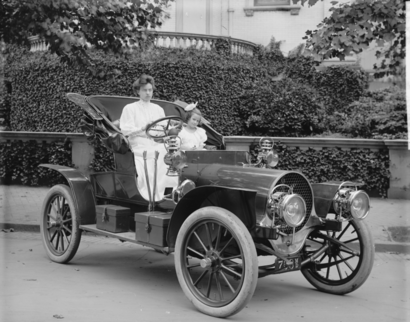
\includegraphics[width=\linewidth]{sample-franklin}
%   \caption{1907 Franklin Model D roadster. Photograph by Harris \&
%     Ewing, Inc. [Public domain], via Wikimedia
%     Commons. (\url{https://goo.gl/VLCRBB}).}
%   \Description{The 1907 Franklin Model D roadster.}
% \end{figure}

% Your figures should contain a caption which describes the figure to
% the reader. Figure captions go below the figure. Your figures should
% {\bfseries also} include a description suitable for screen readers, to
% assist the visually-challenged to better understand your work.

% Figure captions are placed {\itshape below} the figure.

% \subsection{The ``Teaser Figure''}

% A ``teaser figure'' is an image, or set of images in one figure, that
% are placed after all author and affiliation information, and before
% the body of the article, spanning the page. If you wish to have such a
% figure in your article, place the command immediately before the
% \verb|\maketitle| command:
% \begin{verbatim}
%   \begin{teaserfigure}
%     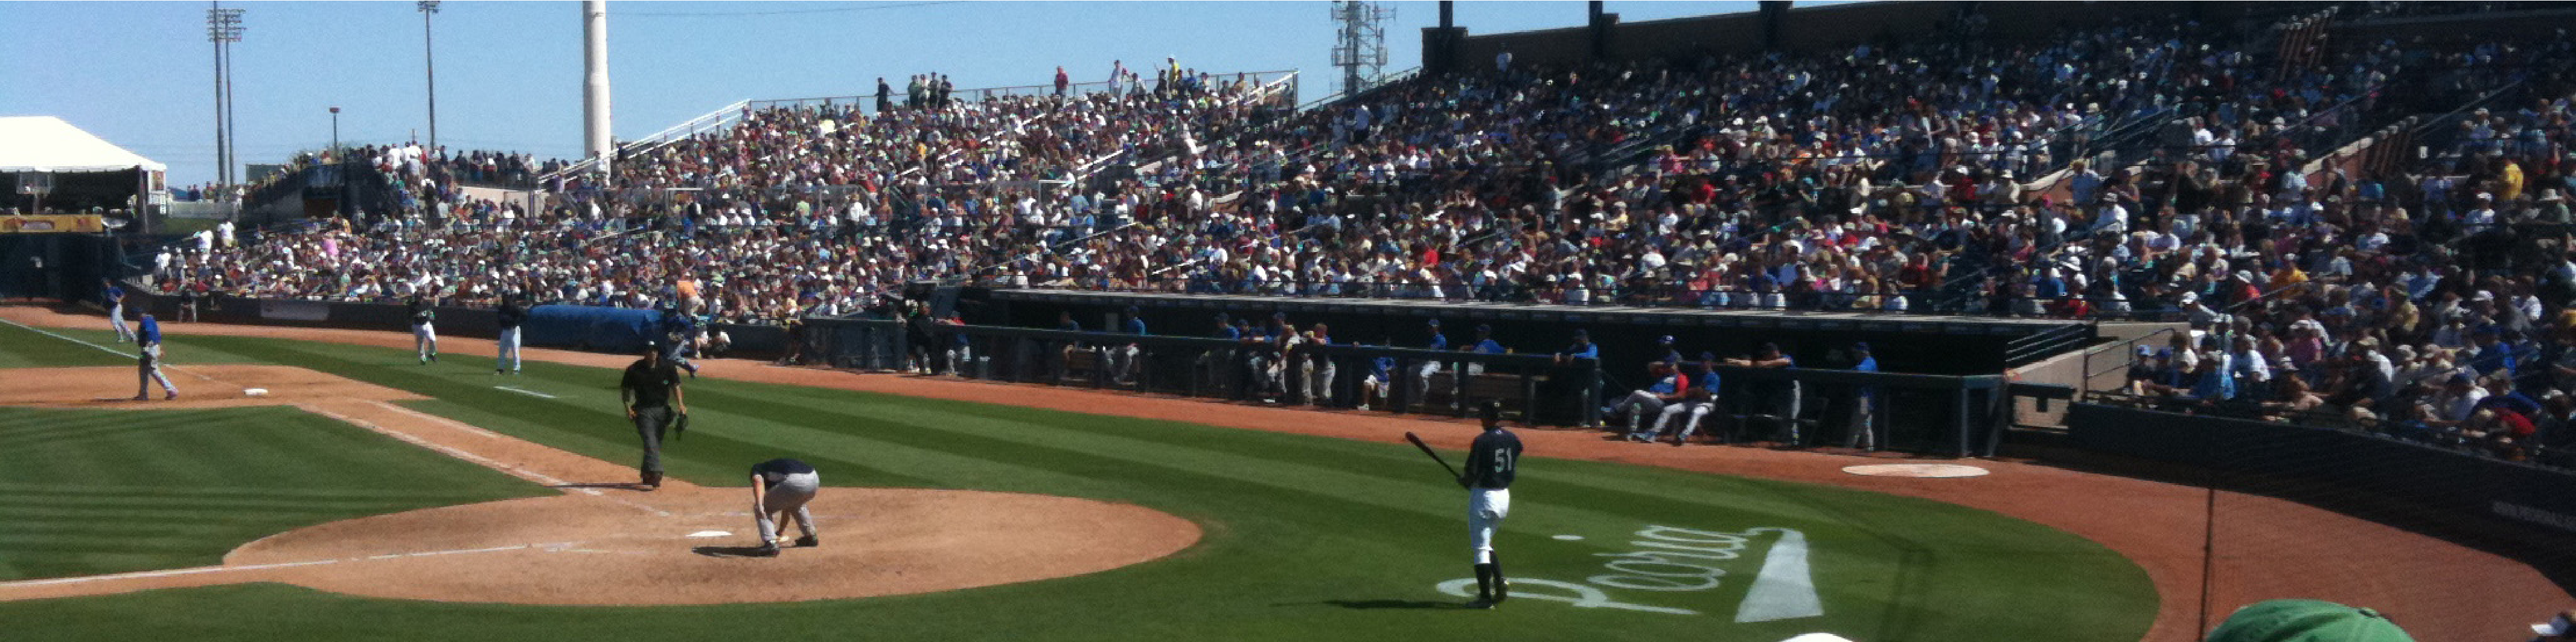
\includegraphics[width=\textwidth]{sampleteaser}
%     \caption{figure caption}
%     \Description{figure description}
%   \end{teaserfigure}
% \end{verbatim}

% \section{Citations and Bibliographies}

% The use of \BibTeX\ for the preparation and formatting of one's
% references is strongly recommended. Authors' names should be complete
% --- use full first names (``Donald E. Knuth'') not initials
% (``D. E. Knuth'') --- and the salient identifying features of a
% reference should be included: title, year, volume, number, pages,
% article DOI, etc.

% The bibliography is included in your source document with these two
% commands, placed just before the \linebreak \verb|\end{document}| command:
% \begin{verbatim}
%   \bibliographystyle{ACM-Reference-Format}
%   \bibliography{bibfile}
% \end{verbatim}
% where ``\verb|bibfile|'' is the name, without the ``\verb|.bib|''
% suffix, of the \BibTeX\ file.

% Citations and references are numbered by default. A small number of
% ACM publications have citations and references formatted in the
% ``author year'' style; for these exceptions, please include this
% command in the {\bfseries preamble} (before \linebreak
% ``\verb|\begin{document}|'') of your \LaTeX\ source:
% \begin{verbatim}
%   \citestyle{acmauthoryear}
% \end{verbatim}

%   Some examples.  A paginated journal article \cite{Abril07}, an
%   enumerated journal article \cite{Cohen07}, a reference to an entire
%   issue \cite{JCohen96}, a monograph (whole book) \cite{Kosiur01}, a
%   monograph/whole book in a series (see 2a in spec. document)
%   \cite{Harel79}, a divisible-book such as an anthology or compilation
%   \cite{Editor00} followed by the same example, however we only output
%   the series if the volume number is given \cite{Editor00a} (so
%   Editor00a's series should NOT be present since it has no vol. no.),
%   a chapter in a divisible book \cite{Spector90}, a chapter in a
%   divisible book in a series \cite{Douglass98}, a multi-volume work as
%   book \cite{Knuth97}, an article in a proceedings (of a conference,
%   symposium, workshop for example) (paginated proceedings article)
%   \cite{Andler79}, a proceedings article with all possible elements
%   \cite{Smith10}, an example of an enumerated proceedings article
%   \cite{VanGundy07}, an informally published work \cite{Harel78}, a
%   doctoral dissertation \cite{Clarkson85}, a master's thesis:
%   \cite{anisi03}, an online document / world wide web resource
%   \cite{Thornburg01, Poker06}, a video game (Case 1)
%   \cite{Obama08} and (Case 2) \cite{Novak03} and \cite{Lee05} and
%   (Case 3) a patent \cite{JoeScientist001}, work accepted for
%   publication \cite{rous08}, 'YYYYb'-test for prolific author
%   \cite{SaeediMEJ10} and \cite{SaeediJETC10}. Other cites might
%   contain 'duplicate' DOI and URLs (some SIAM articles)
%   \cite{Kirschmer:2010:AEI:1958016.1958018}. Boris / Barbara Beeton:
%   multi-volume works as books \cite{MR781536} and \cite{MR781537}. A
%   couple of citations with DOIs:
%   \cite{2004:ITE:1009386.1010128,Kirschmer:2010:AEI:1958016.1958018}. Online
%   citations: \cite{TUGInstmem, Thornburg01, CTANacmart}.

% \section{Acknowledgments}

% Identification of funding sources and other support, and thanks to
% individuals and groups that assisted in the research and the
% preparation of the work should be included in an acknowledgment
% section, which is placed just before the reference section in your
% document.

% This section has a special environment:
% \begin{verbatim}
%   \begin{acks}
%   ...
%   \end{acks}
% \end{verbatim}
% so that the information contained therein can be more easily collected
% during the article metadata extraction phase, and to ensure
% consistency in the spelling of the section heading.

% Authors should not prepare this section as a numbered or unnumbered {\verb|\section|}; please use the ``{\verb|acks|}'' environment.

% \section{Appendices}

% If your work needs an appendix, add it before the \linebreak
% ``\verb|\end{document}|'' command at the conclusion of your source
% document.

% Start the appendix with the ``\verb|appendix|'' command:
% \begin{verbatim}
%   \appendix
% \end{verbatim}
% and note that in the appendix, sections are lettered, not
% numbered. This document has two appendices, demonstrating the section
% and subsection identification method.


%%
%% The acknowledgments section is defined using the "acks" environment
%% (and NOT an unnumbered section). This ensures the proper
%% identification of the section in the article metadata, and the
%% consistent spelling of the heading.
\begin{acks}
%To Robert, for the bagels and explaining CMYK and color spaces.
\end{acks}

%%
%% The next two lines define the bibliography style to be used, and
%% the bibliography file.

\balance
\bibliographystyle{ACM-Reference-Format}
% \bibliography{sample-base}
\bibliography{references}

%%
%% If your work has an appendix, this is the place to put it.
\appendix

% \section{Research Methods}

% \subsection{Part One}

% Lorem ipsum dolor sit amet, consectetur adipiscing elit. Morbi
% malesuada, quam in pulvinar varius, metus nunc fermentum urna, id
% sollicitudin purus odio sit amet enim. Aliquam ullamcorper eu ipsum
% vel mollis. Curabitur quis dictum nisl. Phasellus vel semper risus, et
% lacinia dolor. Integer ultricies commodo sem nec semper.

% \subsection{Part Two}

% Etiam commodo feugiat nisl pulvinar pellentesque. Etiam auctor sodales
% ligula, non varius nibh pulvinar semper. Suspendisse nec lectus non
% ipsum convallis congue hendrerit vitae sapien. Donec at laoreet
% eros. Vivamus non purus placerat, scelerisque diam eu, cursus
% ante. Etiam aliquam tortor auctor efficitur mattis.

% \section{Online Resources}

% Nam id fermentum dui. Suspendisse sagittis tortor a nulla mollis, in
% pulvinar ex pretium. Sed interdum orci quis metus euismod, et sagittis
% enim maximus. Vestibulum gravida massa ut felis suscipit
% congue. Quisque mattis elit a risus ultrices commodo venenatis eget
% dui. Etiam sagittis eleifend elementum.

% Nam interdum magna at lectus dignissim, ac dignissim lorem
% rhoncus. Maecenas eu arcu ac neque placerat aliquam. Nunc pulvinar
% massa et mattis lacinia.

\end{document}
\endinput
%%
%% End of file `sample-sigconf.tex'.
